\documentclass[11pt]{article}

\usepackage[margin=2.4cm]{geometry}
\usepackage[T1]{fontenc}
\usepackage{lmodern}
\usepackage{amsmath,amssymb,amsthm}
\usepackage{booktabs}
\usepackage{multirow}
\usepackage{array}
\usepackage{xcolor}
\usepackage{tikz}
\usetikzlibrary{arrows.meta,positioning,fit,calc}
\usepackage{algorithm}
\usepackage{algpseudocode}
\usepackage{graphicx}
\usepackage[hidelinks]{hyperref}
\usepackage{xurl}

\newtheorem{proposition}{Proposition}
\newcommand{\R}{\mathbb{R}}
\newcommand{\DWT}{\operatorname{DWT}}
\newcommand{\IDWT}{\operatorname{IDWT}}
\newcommand{\IoU}{\operatorname{IoU}}
\newcommand{\pp}{\phantom{+}}

\title{Does a Wavelet Front-End Help a ResNeXt Segment Roads?\\[0.3em]
\large A Controlled Ablation on Massachusetts Roads and DeepGlobe\\
\normalsize Technical report: architecture, equations, protocol and results}
\author{}
\date{October 2026}

\begin{document}
\maketitle

\begin{abstract}
We test, under controlled conditions, whether decomposing the input of a ResNeXt-50 road
segmentation network with a single-level Haar discrete wavelet transform (DWT) improves road
extraction. Four model variants (``rungs'') share one architecture, one training recipe and one
set of seeds, and differ only in how spatial resolution is reduced and restored: R0, a stock
ImageNet-pretrained ResNeXt-50 U-Net; R1, the same network fed a 12-channel Haar decomposition
(the proposed method); R2, learned Haar-basis pooling and unpooling at every resolution change;
and R3, R2 trained with an added soft-clDice topology loss. U-Net and D-LinkNet serve as external
baselines. We give an exact, function-preserving initialisation of the DWT-input stem from the
pretrained weights, which makes R1 identical to R0 at the start of training, and show that a DWT
followed by a convolution is a reparameterisation of a strided convolution. Across 36 runs
(6 models $\times$ 2 datasets $\times$ 3 seeds) and a pre-specified analysis with a seed-aware
bootstrap, the primary comparison R1 $-$ R0 in per-image test IoU is $+0.0004$
(95\% CI $[-0.0040, +0.0060]$) on Massachusetts Roads and $+0.0017$ ($[-0.0018, +0.0059]$) on
DeepGlobe: no detected difference on either dataset.
\end{abstract}

\tableofcontents
\newpage

%=====================================================================================
\section{Question and design}
%=====================================================================================

The proposal under test decomposes each colour channel of the input with a single-level 2D
Haar DWT, stacks the resulting 12 sub-bands, and feeds them to a ResNeXt encoder whose first
convolution is widened from 3 to 12 input channels. The claim is that the sub-bands expose edge
and texture information that helps the network find thin, occluded roads.

To make the effect of the DWT measurable, every variant below shares the encoder backbone, the
decoder, the training data stream, the optimiser, the schedule, the loss (except R3) and the
evaluation. They differ only in the operators that change spatial resolution.

\begin{table}[h]
\centering
\caption{The ablation ladder. All rungs use an ImageNet-pretrained ResNeXt-50 $32{\times}4$d encoder and the same U-Net decoder.}
\label{tab:ladder}
\resizebox{\textwidth}{!}{%
\begin{tabular}{@{}lllll@{}}
\toprule
Rung & Encoder downsampling & Decoder upsampling & Loss & Role \\
\midrule
R0 & strided conv + max-pool (stock) & bilinear + $3{\times}3$ conv & BCE + Dice & control \\
R1 & Haar DWT at the input, stride-1 stem & bilinear + $3{\times}3$ conv & BCE + Dice & \textbf{proposed method} \\
R2 & learned Haar-basis pooling everywhere & learned Haar-basis unpooling + $3{\times}3$ conv & BCE + Dice & strong wavelet variant \\
R3 & as R2 & as R2 & BCE + Dice + $\tfrac12$clDice & connectivity variant \\
\midrule
U-Net & --- & --- & BCE + Dice & external baseline (from scratch) \\
D-LinkNet & --- & --- & BCE + Dice & external baseline (ResNet-34) \\
\bottomrule
\end{tabular}}
\end{table}

\paragraph{Pre-specified primary analysis.} The primary quantity is R1 $-$ R0 in per-image test
IoU at the validation-selected threshold, estimated with a two-level bootstrap that resamples
seeds within each arm and then images (Section~\ref{sec:stats}). A difference is claimed only if
both this interval and a seed-paired $t$ interval exclude zero with the same sign. Everything
else is secondary and reported without multiplicity correction. The plan and the rule were
committed to the code repository before any test score was read.

%=====================================================================================
\section{Datasets}
\label{sec:data}
%=====================================================================================

\subsection{Massachusetts Roads}

Aerial RGB imagery of Massachusetts at 1\,m per pixel, in $1500\times1500$ tiles with binary road
masks rasterised from OpenStreetMap centre-lines \cite{mnih2013}. The official split is used:
1108 training, 14 validation and 49 test tiles.

\begin{itemize}
  \item Original source (used here): \url{https://www.cs.toronto.edu/~vmnih/data/}
  \item Kaggle mirror: \url{https://www.kaggle.com/datasets/balraj98/massachusetts-roads-dataset}
\end{itemize}

\paragraph{No-data regions.} Many tiles contain large blank white areas where no imagery exists.
In a 40-image sample they covered 11\% of pixels on average (over 30\% in 7 images, up to 79\%),
and the labels have roads drawn through them. A pixel is treated as no-data if all three channels
are $\ge 250$ \emph{and} it belongs to a 4-connected white region of at least 2500 pixels; isolated
bright pixels (roofs, lane paint) are kept. The resulting validity mask $V$ is applied to the
training loss, to crop sampling, to checkpoint and threshold selection, and to every metric.
Consequently Massachusetts scores here are \emph{not} directly comparable with published numbers
that count those pixels.

\subsection{DeepGlobe Road Extraction}

Satellite RGB imagery at 0.5\,m per pixel from Thailand, Indonesia and India, in $1024\times1024$
tiles \cite{demir2018}. Only the 6226 training tiles of the challenge were released with masks; the
challenge's validation and test tiles have no public labels. We therefore re-split the 6226
labelled tiles by image into 70/15/15\% with a fixed seed (1337): 4358 training, 933 validation
and 935 test tiles. The test split is pinned by the SHA-256 of its sorted, newline-joined tile ids:
\begin{center}
\footnotesize\ttfamily a18e6da5754390b186234dbe6ba98357\,a1618c9a03d12688a0bdc4fbf65883fe
\end{center}
DeepGlobe has no no-data regions, so $V \equiv 1$.

\begin{itemize}
  \item Challenge page: \url{http://deepglobe.org/}
  \item Kaggle release: \url{https://www.kaggle.com/datasets/balraj98/deepglobe-road-extraction-dataset}
  \item Mirror used here (no Kaggle credentials were available): \url{https://huggingface.co/datasets/lammtfkday/deepglobe-roads}.
        Its counts, tile size and resolution match the original; pixel identity with the Kaggle
        release was not verified. The mirror's own 5000/600/626 partition is not used.
\end{itemize}

\begin{table}[h]
\centering
\caption{Data used in the experiments.}
\begin{tabular}{@{}lccccc@{}}
\toprule
Dataset & Tile size & GSD & Train / val / test & Road pixels & No-data masking \\
\midrule
Massachusetts Roads & $1500^2$ & 1.0 m & 1108 / 14 / 49 & $\approx$5\% of valid & yes \\
DeepGlobe & $1024^2$ & 0.5 m & 4358 / 933 / 935 & $\approx$3.6\% & no \\
\bottomrule
\end{tabular}
\end{table}

\paragraph{No resizing.} Imagery is never resized: roads are 2--4 pixels wide, and downsampling
would delete exactly the structures under study. Training uses $512\times512$ crops; evaluation
tiles each image and stitches the predictions back to full resolution (Section~\ref{sec:eval}).

%=====================================================================================
\section{Architecture}
\label{sec:arch}
%=====================================================================================

\subsection{The Haar transform as fixed convolutions}

Let $\ell = \tfrac{1}{\sqrt2}(1,1)$ and $h = \tfrac{1}{\sqrt2}(1,-1)$. The four $2\times2$ analysis
kernels are the outer products
\begin{equation}
  \kappa_{LL} = \ell^\top\ell,\quad \kappa_{LH} = h^\top\ell,\quad
  \kappa_{HL} = \ell^\top h,\quad \kappa_{HH} = h^\top h,
\end{equation}
so for a $2\times2$ pixel block $\begin{pmatrix} a & b \\ c & d\end{pmatrix}$ the coefficients are
\begin{equation}
\label{eq:haar}
  \mathrm{LL} = \tfrac{a+b+c+d}{2},\quad
  \mathrm{LH} = \tfrac{a+b-c-d}{2},\quad
  \mathrm{HL} = \tfrac{a-b+c-d}{2},\quad
  \mathrm{HH} = \tfrac{a-b-c+d}{2}.
\end{equation}
The four kernels form an orthonormal basis of $\R^{2\times2}$. Applied channel-wise with stride 2,
\begin{equation*}
  \DWT:\ \R^{C\times H\times W}\to\R^{4C\times \frac H2\times\frac W2}
\end{equation*}
is a grouped convolution with frozen weights; channel order is $[c\text{-LL}, c\text{-LH}, c\text{-HL}, c\text{-HH}]$ for each
input channel $c$. Its inverse $\IDWT$ is the adjoint (transposed) convolution with the same
kernels and is exact: $\IDWT(\DWT(x)) = x$. Both run on the GPU inside the network.

\subsection{Encoder}

The encoder is ResNeXt-50 $32\times4$d \cite{xie2017}. Each bottleneck block computes
\begin{equation}
  y = x + \sum_{i=1}^{C} \mathcal{T}_i(x),\qquad C = 32,
\end{equation}
implemented as a $1\times1$ reduction, a $3\times3$ convolution with 32 groups, and a $1\times1$
expansion. The cardinality $C=32$ is the same in every stage; what grows per stage is the width.
For a $512\times512$ input the five feature maps passed to the decoder are:

\begin{table}[h]
\centering
\begin{tabular}{@{}lccc@{}}
\toprule
Feature & Produced by & Resolution & Channels \\
\midrule
$f_0$ & stem & $256^2$ & 64 \\
$f_1$ & layer1 & $128^2$ & 256 \\
$f_2$ & layer2 & $64^2$ & 512 \\
$f_3$ & layer3 & $32^2$ & 1024 \\
$f_4$ & layer4 (bottleneck) & $16^2$ & 2048 \\
\bottomrule
\end{tabular}
\end{table}

\subsection{R1: the DWT-input stem, and an exact initialisation}

\paragraph{Stride parity.} The DWT already halves the resolution, so R1's stem convolution has
stride 1:
\begin{align*}
  \text{R0:}&\quad x\in\R^{3\times512^2} \xrightarrow{\;\text{conv}\,7{\times}7,\ s=2\;} \R^{64\times256^2}
                  \xrightarrow{\;\text{pool},\ s=2\;} \R^{64\times128^2}\\
  \text{R1:}&\quad x \xrightarrow{\;\DWT\;} \R^{12\times256^2}
                  \xrightarrow{\;\text{conv}\,7{\times}7,\ s=1\;} \R^{64\times256^2}
                  \xrightarrow{\;\text{pool},\ s=2\;} \R^{64\times128^2}.
\end{align*}
Every later feature map, skip connection and the whole decoder then have identical shapes in R0
and R1, and the output resolution equals the input resolution (asserted in the code).

\paragraph{Weight adaptation.} Widening the stem from 3 to 12 input channels discards its
ImageNet weights unless they are adapted. The natural adaptation --- give each colour's LL band
the pretrained kernel (halved, since $\mathrm{LL}$ is twice the local mean) and zero the other
bands --- is \emph{not} equivalent to R0: it is the pretrained kernel applied at stride 1 to a
$2\times2$-average-pooled image. An exact adaptation exists.

\begin{proposition}[Exact DWT-domain stem]
\label{prop:exact}
Let $W\in\R^{O\times3\times7\times7}$ be R0's stem kernel (stride 2, padding 3). Let
$K\in\R^{O\times3\times8\times8}$ be $W$ zero-padded by one row at the top and one column at the
left, and $G = \DWT(K)\in\R^{O\times12\times4\times4}$ (the same Haar analysis applied to the
kernel). Define $W'\in\R^{O\times12\times7\times7}$ by $W'[:,:,1{:}5,1{:}5] = G$ and zero elsewhere.
Then for every input $x$ with even height and width,
\begin{equation}
  \mathrm{conv}_{s=1,\,p=3}\big(\DWT(x);\,W'\big) \;=\; \mathrm{conv}_{s=2,\,p=3}\big(x;\,W\big).
\end{equation}
\end{proposition}

\begin{proof}[Sketch]
R0 computes, and after padding equivalently,
\begin{equation*}
  y_{o,i,j} = \sum_{c,u,v} W_{o,c,u,v}\,x_{c,\,2i+u-3,\,2j+v-3}
            = \sum_{c,p,q} K_{o,c,p,q}\,x_{c,\,2i+p-4,\,2j+q-4},\qquad p,q\in\{0,\dots,7\}.
\end{equation*}
Writing $p = 2m+r$, $q=2n+s$ with $m,n\in\{0,\dots,3\}$ and $r,s\in\{0,1\}$, the sum runs over the
$4\times4$ whole $2\times2$ blocks $\beta = (i+m-2,\,j+n-2)$ of the image. Within a block, the
inner product of the kernel block with the pixel block equals the inner product of their Haar
coefficients, because the Haar basis is orthonormal. Hence
\begin{equation*}
  y_{o,i,j} = \sum_{c,k,m,n} G_{o,4c+k,m,n}\;\DWT(x)_{4c+k,\;i+m-2,\;j+n-2},
\end{equation*}
a $4\times4$ stride-1 convolution on the coefficient map; block offsets $-2,\dots,+1$ are taps $1,\dots,4$ of a
$7\times7$ kernel with padding 3. Zero padding agrees on both sides because, with even image
dimensions, every block lies wholly inside or wholly outside the image.
\end{proof}

With this initialisation R1 is the \emph{same function} as the pretrained R0 at step 0 (verified
numerically: maximum logit difference $1.5\times10^{-8}$ on the real launch path). R1 can depart
from R0 only by learning; its stem has $12\cdot49\cdot64 = 37{,}632$ weights against R0's 9408, i.e.\
it can represent a $14\times14$-pixel footprint where R0 has $7\times7$.

\paragraph{Interpretation.} Proposition~\ref{prop:exact} shows that ``DWT, then convolution'' can
represent any strided convolution of the input, and conversely a stride-1 convolution over Haar
sub-bands is a strided convolution with a larger footprint. The DWT front-end therefore does not
add information; it changes the parameterisation and the receptive field of the first layer.

\subsection{R2: learned Haar-basis pooling and unpooling}

\paragraph{WaveletPool.} For $x\in\R^{C\times H\times W}$ with sub-bands
$D = \DWT(x)\in\R^{4C\times\frac H2\times\frac W2}$,
\begin{equation}
  \mathrm{WP}(x)_c = \sum_{k=0}^{3} \omega_{c,k}\, D_{4c+k},\qquad \omega\in\R^{C\times4},
\end{equation}
a learned per-channel $2\times2$ analysis filter expressed in the Haar basis ($4C$ parameters, no
channel mixing). By Eq.~\eqref{eq:haar}, the initialisation $\omega_{c} = (\tfrac12,0,0,0)$ gives
$2\times2$ average pooling, and $\omega_c = (\tfrac12,\tfrac12,\tfrac12,\tfrac12)$ gives
$\tfrac12(\mathrm{LL}+\mathrm{LH}+\mathrm{HL}+\mathrm{HH}) = a$, the top-left pixel of each block,
which is exactly what a stride-2 $1\times1$ convolution reads.

\paragraph{Placement.} In R2 every stride-2 operation of the encoder is replaced by a WaveletPool
placed \emph{in front of the original pretrained layer}, whose stride is set to 1:
\begin{center}
\begin{tabular}{@{}lll@{}}
\toprule
Replaced operation & Becomes & Initialisation (exact at step 0?) \\
\midrule
stem max-pool $3{\times}3$, $s=2$ & $\mathrm{WP}_{64}$ & average (no) \\
layer$\{2,3,4\}$.0 grouped $3{\times}3$, $s=2$ & $\mathrm{conv}_{3\times3,s=1}\circ\mathrm{WP}$ & average (no) \\
layer$\{2,3,4\}$.0 shortcut $1{\times}1$, $s=2$ & $\mathrm{conv}_{1\times1,s=1}\circ\mathrm{WP}$ & top-left pixel (\textbf{yes}) \\
\bottomrule
\end{tabular}
\end{center}
All pretrained weights are kept and the cardinality remains 32. At initialisation R2's features
have cosine similarity 1.000, 0.909, 0.931, 0.945, 0.955 to R0's at the five stages.

\paragraph{WaveletUnpool.} In the decoder,
\begin{equation}
  \mathrm{WU}(x) = \IDWT\big([\,\omega_{c,k}\,x_c\,]_{c,k}\big),\qquad \omega_c = (2,0,0,0)\text{ at init},
\end{equation}
which at initialisation is nearest-neighbour upsampling. R2's upsampling block is
$\mathrm{conv}_{3\times3}\circ\mathrm{WU}$, against R0's $\mathrm{conv}_{3\times3}\circ\mathrm{bilinear}$:
the two differ only in the $2\times$ kernel.

\paragraph{Seed pairing.} The wavelet parameters are initialised deterministically and draw
nothing from the random stream, and the decoder and head are constructed before the encoder. At a
fixed seed, every weight shared by two rungs is bitwise identical.

\subsection{Decoder and head}

A U-Net decoder \cite{ronneberger2015} with explicit skip connections:
\begin{equation}
  d_\ell = \phi_\ell\big(\,[\,\mathrm{Up}_\ell(d_{\ell-1})\;;\;f_{4-\ell}\,]\,\big),\qquad d_0 = f_4,
\end{equation}
where $\phi_\ell$ is two $3\times3$ Conv--BN--ReLU layers and $f_{-1}$ is empty (no skip at full
resolution). Widths are 512, 256, 128, 64, 32 at resolutions $32^2,64^2,128^2,256^2,512^2$. A
$1\times1$ convolution produces one logit per pixel; the sigmoid is applied only in the loss and
the metrics.

\begin{figure}[h]
\centering
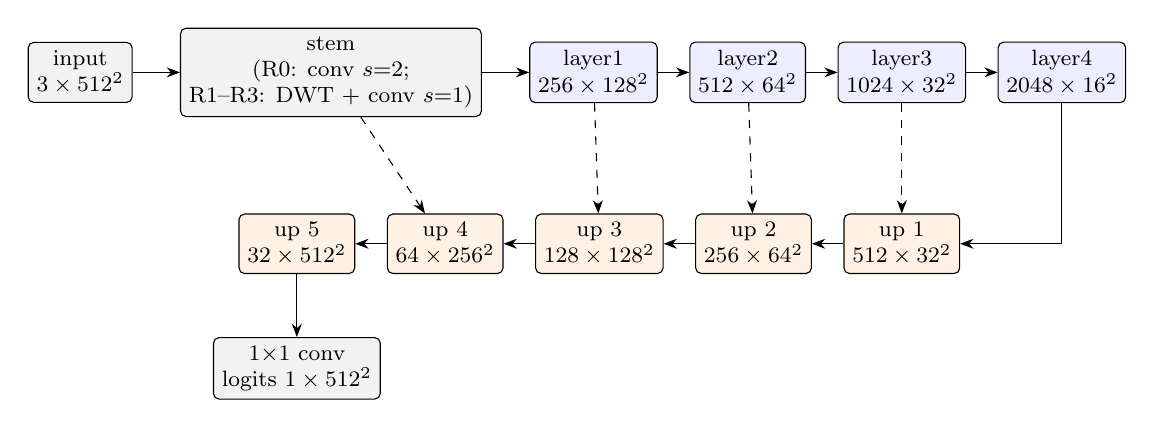
\begin{tikzpicture}[
  font=\footnotesize, >=Stealth,
  box/.style={draw, rounded corners=2pt, minimum height=7mm, align=center, inner sep=3pt},
  enc/.style={box, fill=blue!7}, dec/.style={box, fill=orange!10}, op/.style={box, fill=gray!10}]
\node[op] (in) {input\\$3\times512^2$};
\node[op, right=6mm of in] (stem) {stem\\(R0: conv $s{=}2$;\\R1--R3: DWT + conv $s{=}1$)};
\node[enc, right=6mm of stem] (l1) {layer1\\$256\times128^2$};
\node[enc, right=4mm of l1] (l2) {layer2\\$512\times64^2$};
\node[enc, right=4mm of l2] (l3) {layer3\\$1024\times32^2$};
\node[enc, right=4mm of l3] (l4) {layer4\\$2048\times16^2$};
\draw[->] (in) -- (stem); \draw[->] (stem) -- (l1); \draw[->] (l1) -- (l2);
\draw[->] (l2) -- (l3); \draw[->] (l3) -- (l4);
\node[dec, below=14mm of l3] (d1) {up 1\\$512\times32^2$};
\node[dec, left=4mm of d1] (d2) {up 2\\$256\times64^2$};
\node[dec, left=4mm of d2] (d3) {up 3\\$128\times128^2$};
\node[dec, left=4mm of d3] (d4) {up 4\\$64\times256^2$};
\node[dec, left=4mm of d4] (d5) {up 5\\$32\times512^2$};
\node[op, below=8mm of d5] (out) {$1{\times}1$ conv\\logits $1\times512^2$};
\draw[->] (l4) |- (d1); \draw[->] (d1) -- (d2); \draw[->] (d2) -- (d3);
\draw[->] (d3) -- (d4); \draw[->] (d4) -- (d5); \draw[->] (d5) -- (out);
\draw[->, dashed] (l3) -- (d1); \draw[->, dashed] (l2) -- (d2);
\draw[->, dashed] (l1) -- (d3); \draw[->, dashed] (stem) -- (d4);
\end{tikzpicture}
\caption{The shared encoder--decoder. Dashed arrows are skip connections. R0 and R1 upsample
bilinearly; R2 and R3 replace every stride-2 encoder operation by WaveletPool and every decoder
upsampling by WaveletUnpool.}
\label{fig:arch}
\end{figure}

\subsection{Parameter counts}

\begin{table}[h]
\centering
\caption{Trainable parameters (exact). The wavelet rungs add 0.06--0.12\% to R0.}
\label{tab:params}
\begin{tabular}{@{}lrrr@{}}
\toprule
Model & Encoder & Decoder + head & Total \\
\midrule
R0 & 22{,}979{,}904 & 23{,}523{,}233 & 46{,}503{,}137 \\
R1 & 23{,}008{,}128 & 23{,}523{,}233 & 46{,}531{,}361 \\
R2, R3 & 23{,}022{,}720 & 23{,}535{,}265 & 46{,}557{,}985 \\
U-Net (from scratch) & \multicolumn{2}{c}{---} & 31{,}037{,}633 \\
D-LinkNet (ResNet-34) & \multicolumn{2}{c}{---} & 31{,}095{,}137 \\
\bottomrule
\end{tabular}
\end{table}

\paragraph{Baselines.} U-Net: four levels of widths 64--512 with a 1024-wide bottleneck, trained
from scratch. D-LinkNet \cite{zhou2018}: ResNet-34 encoder (ImageNet), a centre block of
\emph{cascaded} dilated $3\times3$ convolutions with dilations 1, 2, 4, 8 whose outputs are summed
with the input ($d_1 = \rho(c_1(x)),\ d_{k+1} = \rho(c_{k+1}(d_k)),\ \text{out} = x + \sum_k d_k$),
and a LinkNet decoder with additive skips.

%=====================================================================================
\section{Training}
\label{sec:train}
%=====================================================================================

\subsection{Loss}

Let $z$ be the logits, $p = \sigma(z)$, $y\in\{0,1\}$ the mask and $m\in\{0,1\}$ the validity mask,
for one $512\times512$ crop; sums run over pixels.
\begin{align}
  \mathcal{L}_{\mathrm{BCE}} &= \frac{\sum m\,\mathrm{bce}(z,y)}{\max(\sum m,\,1)}
  \quad\text{(normalised over the valid pixels of the whole batch)},\\
  \mathcal{L}_{\mathrm{Dice}} &= 1 - \frac{2\sum p\,y\,m + 1}{\sum p\,m + \sum y\,m + 1}
  \quad\text{(per sample, averaged over the batch)}.
\end{align}
R0, R1, R2 and both baselines minimise $\mathcal{L}_{\mathrm{BCE}} + \mathcal{L}_{\mathrm{Dice}}$.
The Dice smoothing constant 1 keeps road-free crops (the majority) numerically stable.

\paragraph{clDice (R3).} With a differentiable soft skeleton $S(\cdot)$ (iterated soft
erosion/dilation by $3\times3$ min/max pooling, 6 iterations \cite{shit2021}), on masked inputs
$\tilde p = p\,m$, $\tilde y = y\,m$:
\begin{equation}
  T_{\mathrm{prec}} = \frac{\sum S(\tilde p)\,\tilde y}{\sum S(\tilde p)+\epsilon},\quad
  T_{\mathrm{sens}} = \frac{\sum S(\tilde y)\,\tilde p}{\sum S(\tilde y)+\epsilon},\quad
  \mathrm{clDice} = \frac{2\,T_{\mathrm{prec}}T_{\mathrm{sens}}}{T_{\mathrm{prec}}+T_{\mathrm{sens}}+\epsilon},
\end{equation}
with $\epsilon=10^{-6}$, and
\begin{equation}
  \mathcal{L}_{\mathrm{R3}} = \mathcal{L}_{\mathrm{BCE}} + \mathcal{L}_{\mathrm{Dice}} + \lambda\,(1-\mathrm{clDice}),\qquad \lambda = 0.5.
\end{equation}
On a road-free crop $S(\tilde y)=0$, so the term equals 1 with zero gradient. All losses are
computed in fp32; the forward pass runs under bf16 autocast.

\subsection{Data pipeline}

\begin{itemize}
  \item \textbf{Crops.} Random $512\times512$ crops, $8\times$ the number of training images per
        epoch (8864 for Massachusetts, 34{,}864 for DeepGlobe). With probability 0.75 a crop is
        resampled (up to 12 tries) until it contains road on valid pixels; crops with less than
        50\% valid pixels are rejected.
  \item \textbf{Augmentation.} Horizontal/vertical flips and $90^\circ$ rotations; with probability
        0.5 an affine warp (rotation $\pm15^\circ$, scale $0.9$--$1.1$, bilinear for the image,
        nearest for the masks, reflective borders); with probability 0.5 brightness and contrast
        jitter in $[0.9, 1.1]$. ImageNet mean/std normalisation is applied once, after augmentation.
  \item \textbf{Pairing.} All randomness comes from one seeded generator per item, and the data
        loader has its own generator: for a given seed, every rung sees the identical crop stream.
\end{itemize}

\subsection{Optimisation}

AdamW, learning rate $\eta_0 = 3\times10^{-4}$, weight decay $10^{-4}$ on all parameters, batch 16,
gradient-norm clipping at 1.0 (a non-finite loss or gradient stops the run). Per-iteration schedule
with $T_w$ warmup steps (2 epochs) out of $T$ total:
\begin{equation}
  \eta(t) =
  \begin{cases}
    \eta_0\big(0.01 + 0.99\,\tfrac{t}{T_w}\big), & t < T_w,\\[4pt]
    \eta_{\min} + \tfrac12(\eta_0-\eta_{\min})\Big(1+\cos\tfrac{\pi(t-T_w)}{T-T_w}\Big), & t \ge T_w,
  \end{cases}
  \qquad \eta_{\min} = 0.01\,\eta_0.
\end{equation}
Massachusetts: 100 epochs of 554 steps ($T = 55{,}400$, $T_w = 1108$). DeepGlobe: 40 epochs of
2179 steps ($T = 87{,}160$, $T_w = 4358$). One recipe for every model; nothing was tuned per rung.

\subsection{Model selection}

After each epoch, the pooled validation IoU is computed at threshold 0.5 on non-overlapping tiles;
the best epoch's weights are kept. After training, the decision threshold is chosen on the
validation split from $\{0.20, 0.25, \dots, 0.80\}$ to maximise pooled IoU. The test split is not
read during training or selection.

%=====================================================================================
\section{Evaluation}
\label{sec:eval}
%=====================================================================================

\subsection{Full-image inference}

Each test image is covered by $512\times512$ tiles at stride 256, with the last row and column
aligned to the image edge (25 tiles per Massachusetts image, 9 per DeepGlobe image). Tile
probabilities are averaged where tiles overlap,
\begin{equation}
  P(u) = \frac{\sum_t \mathbf{1}[u\in t]\,P_t(u)}{\sum_t \mathbf{1}[u\in t]},
\end{equation}
and the prediction is $\hat Y = \{u : P(u) \ge \tau^\ast\}$. All metrics are computed on the
stitched full-resolution image, over valid pixels only. Each run's test split is scored exactly
once; the probability maps are saved.

\subsection{Metrics}

With $\mathrm{TP},\mathrm{FP},\mathrm{FN}$ counted over valid pixels:
\begin{itemize}
  \item \textbf{IoU} $= \mathrm{TP}/(\mathrm{TP}+\mathrm{FP}+\mathrm{FN})$, reported per image
        (mean over images) and pooled (counts summed over images). An image with no valid pixels
        has no score; an all-background prediction on a road-free image scores 1.
  \item \textbf{Relaxed precision/recall/F1} \cite{mnih2010}: a predicted pixel is correct if a
        ground-truth road pixel lies within Euclidean distance $\rho = 3$ px, and vice versa.
  \item \textbf{clDice} (hard skeletons) \cite{shit2021}.
  \item \textbf{APLS} \cite{vanetten2018}: graphs are built from the skeletons of prediction and
        ground truth; for 500 sampled node pairs per direction,
        $\mathrm{APLS} = 1 - \frac1N\sum\min\!\big(1, \frac{|L - \hat L|}{L}\big)$, averaged over
        both directions; a node with no counterpart within 8 px contributes the maximum penalty.
\end{itemize}

%=====================================================================================
\section{Statistical analysis}
\label{sec:stats}
%=====================================================================================

Let $u_{a,s,i}$ be the test IoU of image $i$ for arm $a\in\{0,1\}$ (baseline, comparison) and seed
$s$; $\bar u_{a,i}$ its mean over the arm's seeds; $N$ the number of images. The point estimate is
\begin{equation}
  \hat\Delta = \frac1N\sum_{i=1}^N \big(\bar u_{1,i} - \bar u_{0,i}\big).
\end{equation}

\begin{algorithm}[h]
\caption{Two-level paired bootstrap (primary interval)}
\begin{algorithmic}[1]
\For{$b = 1,\dots,B$ \quad ($B = 10{,}000$, fixed seed)}
  \State draw seeds $S_0^\ast$, $S_1^\ast$ with replacement, independently within each arm
  \State draw image indices $I^\ast$ with replacement (the same draw for both arms)
  \State $\Delta^\ast_b \gets \frac{1}{N}\sum_{i\in I^\ast}\Big(\frac{1}{|S_1^\ast|}\sum_{s\in S_1^\ast}u_{1,s,i} - \frac{1}{|S_0^\ast|}\sum_{s\in S_0^\ast}u_{0,s,i}\Big)$
\EndFor
\State 95\% CI: the 2.5th and 97.5th percentiles of $\{\Delta^\ast_b\}$
\State $p = \min\!\Big(1,\ 2\min\!\Big(\frac{\#\{\Delta^\ast_b\le0\}+1}{B+1},\ \frac{\#\{\Delta^\ast_b\ge0\}+1}{B+1}\Big)\Big)$
\end{algorithmic}
\end{algorithm}

Resampling seeds as well as images targets the training procedure rather than three particular
trained models. With three seeds the interval is crude: in simulation it covered 0.94--0.98 in most
regimes but 0.86 when seed variance dominated at $N=935$.

\paragraph{Seed-paired $t$ interval.} Seeds are paired by design (same crop stream and same
shared initialisation). With $d_s = \frac1N\sum_i (u_{1,s,i}-u_{0,s,i})$ over the $n=3$ common seeds,
the interval is $\bar d \pm t_{0.975,\,n-1}\, s_d/\sqrt n$.

\paragraph{Decision rule (pre-specified).} A difference is claimed only if \emph{both} intervals
exclude zero with the same sign. If exactly one excludes zero, or they exclude it with opposite
signs, the result is \emph{inconclusive} at three seeds (and more seeds would be needed before any
claim). If neither excludes zero: \emph{no detected difference}.

%=====================================================================================
\section{Results}
\label{sec:results}
%=====================================================================================

All 36 runs completed (no failures). Test scores are reported at the validation-selected threshold.

\subsection{Primary comparison}

\begin{table}[h]
\centering
\caption{Primary analysis: R1 (DWT at the input) versus R0 (stock), per-image test IoU, 3 seeds per arm.}
\label{tab:primary}
\resizebox{\textwidth}{!}{%
\begin{tabular}{@{}lcccccc@{}}
\toprule
Dataset & $N$ & R0 pooled IoU & R1 pooled IoU & $\hat\Delta$ & Two-level 95\% CI ($p$) & Seed-paired $t$ 95\% CI \\
\midrule
Massachusetts & 49 & 0.6562 & 0.6554 & $+0.0004$ & $[-0.0040, +0.0060]$ (0.90) & $[-0.0095, +0.0104]$ \\
DeepGlobe & 935 & 0.6771 & 0.6785 & $+0.0017$ & $[-0.0018, +0.0059]$ (0.38) & $[-0.0072, +0.0106]$ \\
\bottomrule
\end{tabular}}
\end{table}

\textbf{Decision: no detected difference on either dataset.} The robustness checks agree: the
difference in pooled IoU is $-0.0008$ $[-0.0044, +0.0032]$ (Massachusetts) and $+0.0015$
$[-0.0013, +0.0045]$ (DeepGlobe); in IoU at a fixed threshold of 0.5 it is $+0.0014$
$[-0.0032, +0.0077]$ and $+0.0018$ $[-0.0017, +0.0061]$. No test image has fewer than 2000 road
pixels on valid pixels, so the near-empty-image sensitivity analysis excludes nothing.

\subsection{Secondary comparisons}

\begin{table}[h]
\centering
\caption{All models against R0 (per-image test IoU). Secondary and exploratory: no multiplicity correction.}
\label{tab:secondary}
\small
\begin{tabular}{@{}llcccl@{}}
\toprule
Dataset & Model & Pooled IoU (mean $\pm$ sd) & $\hat\Delta$ vs R0 & Two-level 95\% CI & Decision \\
\midrule
\multirow{6}{*}{Massachusetts}
 & R0 & $0.6562 \pm 0.0011$ & --- & --- & --- \\
 & R1 & $0.6554 \pm 0.0024$ & $+0.0004$ & $[-0.0040, +0.0060]$ & no difference \\
 & R2 & $0.6545 \pm 0.0001$ & $-0.0009$ & $[-0.0060, +0.0049]$ & no difference \\
 & R3 & $0.6553 \pm 0.0018$ & $-0.0018$ & $[-0.0061, +0.0020]$ & no difference \\
 & U-Net & $0.6632 \pm 0.0001$ & $+0.0095$ & $[+0.0047, +0.0151]$ & difference \\
 & D-LinkNet & $0.6515 \pm 0.0014$ & $-0.0043$ & $[-0.0114, +0.0023]$ & inconclusive \\
\midrule
\multirow{6}{*}{DeepGlobe}
 & R0 & $0.6771 \pm 0.0023$ & --- & --- & --- \\
 & R1 & $0.6785 \pm 0.0010$ & $+0.0017$ & $[-0.0018, +0.0059]$ & no difference \\
 & R2 & $0.6823 \pm 0.0011$ & $+0.0039$ & $[+0.0001, +0.0084]$ & inconclusive$^\dagger$ \\
 & R3 & $0.6743 \pm 0.0013$ & $-0.0027$ & $[-0.0069, +0.0019]$ & no difference \\
 & U-Net & $0.6461 \pm 0.0008$ & $-0.0332$ & $[-0.0381, -0.0277]$ & difference \\
 & D-LinkNet & $0.6655 \pm 0.0005$ & $-0.0081$ & $[-0.0126, -0.0033]$ & inconclusive \\
\bottomrule
\end{tabular}

\vspace{2pt}
{\footnotesize $^\dagger$ The bootstrap interval excludes zero but the seed-paired $t$ interval
$[-0.0059, +0.0137]$ does not (per-seed differences $+0.0033, +0.0003, +0.0082$).}
\end{table}

\subsection{Other metrics (exploratory)}

\begin{table}[h]
\centering
\caption{Mean $\pm$ sd over 3 seeds of per-image test metrics. Exploratory; the metrics are correlated.}
\label{tab:metrics}
\small
\begin{tabular}{@{}llcccc@{}}
\toprule
Dataset & Model & IoU & Relaxed F1 ($\rho{=}3$) & clDice & APLS \\
\midrule
\multirow{6}{*}{Massachusetts}
 & R0 & $0.6529\pm0.0008$ & $0.9072\pm0.0011$ & $0.8812\pm0.0012$ & $0.8047\pm0.0041$ \\
 & R1 & $0.6533\pm0.0032$ & $0.9087\pm0.0037$ & $0.8821\pm0.0036$ & $0.8029\pm0.0040$ \\
 & R2 & $0.6520\pm0.0034$ & $0.9079\pm0.0048$ & $0.8822\pm0.0047$ & $0.8029\pm0.0039$ \\
 & R3 & $0.6511\pm0.0016$ & $0.9060\pm0.0012$ & $0.8828\pm0.0016$ & $0.8040\pm0.0027$ \\
 & U-Net & $0.6624\pm0.0003$ & $0.9155\pm0.0002$ & $0.8895\pm0.0004$ & $0.8006\pm0.0030$ \\
 & D-LinkNet & $0.6486\pm0.0014$ & $0.9080\pm0.0006$ & $0.8806\pm0.0008$ & $0.8002\pm0.0025$ \\
\midrule
\multirow{6}{*}{DeepGlobe}
 & R0 & $0.6751\pm0.0032$ & $0.8978\pm0.0026$ & $0.8665\pm0.0020$ & $0.7755\pm0.0045$ \\
 & R1 & $0.6768\pm0.0005$ & $0.8988\pm0.0004$ & $0.8670\pm0.0007$ & $0.7777\pm0.0020$ \\
 & R2 & $0.6790\pm0.0011$ & $0.8996\pm0.0005$ & $0.8687\pm0.0003$ & $0.7814\pm0.0013$ \\
 & R3 & $0.6723\pm0.0010$ & $0.8952\pm0.0013$ & $0.8683\pm0.0009$ & $0.7763\pm0.0045$ \\
 & U-Net & $0.6419\pm0.0009$ & $0.8764\pm0.0008$ & $0.8378\pm0.0011$ & $0.7193\pm0.0020$ \\
 & D-LinkNet & $0.6669\pm0.0008$ & $0.8955\pm0.0004$ & $0.8613\pm0.0009$ & $0.7614\pm0.0036$ \\
\bottomrule
\end{tabular}
\end{table}

\subsection{Compute}

All 36 runs trained on single NVIDIA L40S GPUs (48 GB) with bf16 autocast. At batch 16 of $512^2$
crops, the GPU self-test measured 3.65--3.89 steps/s for R0--R3 (peak memory 11.9--13.0 GB),
2.97 steps/s for U-Net (17.2 GB) and 9.69 steps/s for D-LinkNet (5.4 GB). A Massachusetts epoch
of R0 took about 132 s including validation ($\approx$3.7 h per run); a DeepGlobe epoch took
9.1--9.9 min ($\approx$6.1--6.6 h per run).

%=====================================================================================
\section{Discussion}
%=====================================================================================

\paragraph{The DWT front-end does not help a pretrained ResNeXt.} On both datasets the primary
interval is narrow and centred near zero; gains larger than about 0.6 IoU points are excluded.
Proposition~\ref{prop:exact} explains why this is unsurprising: a DWT followed by a convolution
is a reparameterised strided convolution with a larger footprint, so it adds no information that
a pretrained first layer lacks. Starting R1 exactly at R0 isolates this effect; with the
non-equivalent ``LL-only'' adaptation, any difference would have been confounded with the loss of
pretrained features.

\paragraph{Learned wavelet pooling throughout (R2).} On DeepGlobe, R2 is ahead of R0 on every
metric (IoU $+0.004$, APLS $+0.006$) with smaller seed-to-seed spread, but the pre-specified rule
classifies it as inconclusive at three seeds, and it shows nothing on Massachusetts. R2 replaces
aliasing strided operations by learned filters that start as averaging, i.e.\ anti-aliased
downsampling \cite{zhang2019,li2021wavecnet}; if it has a benefit, robustness to shifts and
corruptions is the more likely place to find it than clean IoU. Any such test should be specified
before it is run.

\paragraph{Topology loss (R3).} Adding soft-clDice did not improve IoU, clDice or APLS on either
dataset.

\paragraph{Baselines.} The from-scratch U-Net is the best model on Massachusetts but the worst on
DeepGlobe, suggesting that ImageNet pretraining matters less on Massachusetts' smaller training
set and near-constant-width centre-line labels than on DeepGlobe's more varied scenes.

%=====================================================================================
\section{Limitations}
%=====================================================================================

\begin{itemize}
  \item Three seeds per model; the headline interval can be anti-conservative when seed variance
        dominates. Only R1 $-$ R0 per-image IoU was pre-specified.
  \item R2 and R3 change the encoder and the decoder operators together.
  \item Only the exact stem initialisation was run; the ``LL-only'' variant was not.
  \item One untuned recipe for every model; weight decay is applied to all parameters including
        BatchNorm.
  \item Checkpoint and threshold are selected per run on validation, which is 14 images for
        Massachusetts.
  \item Massachusetts scores exclude a custom no-data mask and are not comparable with published
        numbers. The DeepGlobe split is our own random split by image (adjacent tiles may fall in
        different splits), and its files come from a mirror whose pixel identity with the original
        release was not verified.
  \item bf16 autocast and non-deterministic GPU kernels: reruns are statistically, not bitwise,
        reproducible (all runs used the same GPU model, the NVIDIA L40S).
  \item Edge-aligned tiling with uniform overlap averaging; no test-time augmentation.
  \item The soft skeleton uses a $3\times3$ square min-pool rather than a cross.
\end{itemize}

%=====================================================================================
\section{Reproducibility}
%=====================================================================================

The experiment ran from a frozen snapshot of the code (commit \texttt{c1d1e2f}) on 12--14 October
2026. Each run directory records the resolved configuration, seed, code commit, library versions,
CUDA/cuDNN versions, the SHA-256 of the pretrained weights, the DeepGlobe split fingerprint,
the training history, the validation-selected threshold, and per-image test scores. The code base
includes a 458-test suite, a CPU end-to-end rehearsal and a GPU self-test; the decisions taken
during implementation, with their reasons, are recorded in \texttt{docs/DECISIONS.md}.

%=====================================================================================
\begin{thebibliography}{99}
\bibitem{mnih2013} V.~Mnih. \emph{Machine Learning for Aerial Image Labeling}. PhD thesis,
  University of Toronto, 2013.
\bibitem{mnih2010} V.~Mnih and G.~E.~Hinton. Learning to detect roads in high-resolution aerial
  images. In \emph{ECCV}, 2010.
\bibitem{demir2018} I.~Demir, K.~Koperski, D.~Lindenbaum, G.~Pang, J.~Huang, S.~Basu, F.~Hughes,
  D.~Tuia, and R.~Raskar. DeepGlobe 2018: A challenge to parse the Earth through satellite images.
  In \emph{CVPR Workshops}, 2018.
\bibitem{xie2017} S.~Xie, R.~Girshick, P.~Doll\'ar, Z.~Tu, and K.~He. Aggregated residual
  transformations for deep neural networks. In \emph{CVPR}, 2017.
\bibitem{mallat1989} S.~G.~Mallat. A theory for multiresolution signal decomposition: the wavelet
  representation. \emph{IEEE TPAMI}, 11(7):674--693, 1989.
\bibitem{ronneberger2015} O.~Ronneberger, P.~Fischer, and T.~Brox. U-Net: Convolutional networks
  for biomedical image segmentation. In \emph{MICCAI}, 2015.
\bibitem{zhou2018} L.~Zhou, C.~Zhang, and M.~Wu. D-LinkNet: LinkNet with pretrained encoder and
  dilated convolution for high resolution satellite imagery road extraction. In
  \emph{CVPR Workshops}, 2018.
\bibitem{shit2021} S.~Shit, J.~C.~Paetzold, A.~Sekuboyina, I.~Ezhov, A.~Unger, A.~Zhylka,
  J.~P.~W.~Pluim, U.~Bauer, and B.~H.~Menze. clDice -- a novel topology-preserving loss function
  for tubular structure segmentation. In \emph{CVPR}, 2021.
\bibitem{vanetten2018} A.~Van~Etten, D.~Lindenbaum, and T.~M.~Bacastow. SpaceNet: A remote sensing
  dataset and challenge series. \emph{arXiv:1807.01232}, 2018.
\bibitem{zhang2019} R.~Zhang. Making convolutional networks shift-invariant again. In
  \emph{ICML}, 2019.
\bibitem{li2021wavecnet} Q.~Li, L.~Shen, S.~Guo, and Z.~Lai. WaveCNet: Wavelet integrated CNNs to
  suppress aliasing effect for noise-robust image classification. \emph{IEEE TIP}, 30:7074--7089, 2021.
\bibitem{liu2018mwcnn} P.~Liu, H.~Zhang, K.~Zhang, L.~Lin, and W.~Zuo. Multi-level wavelet-CNN for
  image restoration. In \emph{CVPR Workshops}, 2018.
\end{thebibliography}

\end{document}
